\documentclass{article}
\usepackage{listings}
\usepackage{amsmath}
\usepackage{graphicx}
\usepackage{float}
\usepackage{subcaption}
\usepackage[linewidth=1pt]{mdframed}
\usepackage[colorlinks]{hyperref}

\usepackage{algorithm}
\usepackage{algpseudocode}

\hypersetup{citecolor=DeepPink4}
\hypersetup{linkcolor=DarkRed}
\hypersetup{urlcolor=Blue}

\usepackage{cleveref}

\setlength{\parindent}{1em}
\setlength{\parskip}{1em}
\renewcommand{\baselinestretch}{1.0}

\begin{document}

\begin{titlepage}
	\centering
	{\scshape\LARGE Assignment 2\par}
	\vspace{1cm}
	{\scshape\Large Algorithms \& Complexity (CIS 522-01)\par}
	\vspace{1.5cm}
	{\Large\itshape Javier Arechalde\par}
	\vfill
	{\large \today\par}
\end{titlepage}

\section*{Stress Testing}

\subsection*{Model description}

In this problem, we are doing some stress-testing on various models of glass jars, to determine the highest distance they can be dropped without breaking. 

We have a ladder with $n$ rungs, and we want to find the \textit{highest safe rung}, that is the distance that we described in the last paragraph. We also have $k$ jars, and this number of available jars, will be limited depending on the "budget" for the test.

\subsection*{a.}

In this case our budget is limited to $k = 2$ and we want to find a solution $f(n)$ that grows slower than linearly. The breaking distance for the first jar $k_1$ is $bd$ and the breaking distance for the second jar $k_2$ is $bd$ too, as they are models of the same jar.

The current rung we are dropping our jars from is $r$, and the highest safe run will be assigned to $sr$.

\subsection*{Overall idea}

In case we are given 2 jars, $k = 2$, we will use one algorithm with a different approach, because if we use linear search, our solution will grow linearly, but if we use binary search, we will exceed the number of available jars we have for this problem.

So in our solution, we will divide the ladder into $m$ divisions. This way, our algorithm will take $(m+n/m)$ steps at most. This can be explained because in the worst case scenario, we will need to go over all the $m$ divisions to find the highest safe rung, and then go to the start of the previous division before it broke, and go to the next division, which is $n/m$ steps away from the previous division.

\subsection*{Pseudocode}

\begin{algorithm}[H]
\caption{My implementation}
\begin{algorithmic}[1]
\State At the beginning $r = 0$ and $k_1,k_2$ are not broken
\State We have $n$ rungs, and we chose to divide our rungs into $m = 4$
\While{$k_1$ not broken}
 \State Start increasing distance
 \State Saving last ring $r_0 = r$
 \State $r = r + n/m$
 \If{$r>bd$}
  \State $k_1$ breaks at rung r
 \EndIf
\EndWhile
\State We start our next iterations from r = r0
\While{$k_2$ not broken}
 \State r = r + 1
 \If{$r>bd$}
  \State We return $sr = r-1$, safest rung distance for the jars not to break
 \EndIf 
\EndWhile
\end{algorithmic}
\end{algorithm}

\subsection*{Example}

Now, we will prove that our algorithm works, by implementing it and running it.

\lstinputlisting[language=Python]{Problem1a.py}

In the image shown below, you can see the results of running this algorithm, in an example setup.

\begin{figure}[H]
\begin{center}
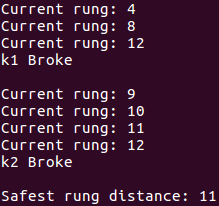
\includegraphics[scale=.8]{problem1a}
\end{center}
\caption{Results of running algorithm}
\end{figure}

\subsection*{Time complexity analysis}

\subsection*{b.}

In this case, out budget is limited to $k$ jars, where $k>2$. We want to find the highest safe rung using at most $k$ jars. For each jar $k_i$ the number of times we drop whis jar should be less than the number of times we dropped the previous jar $k_{i-1}$ so $\lim_{n\to\infty} f_k(n)/f_{k-1}(n) = 0$.

The current rung we are dropping our jars from is $r$, and the highest safe run will be assigned to $sr$.

\subsection*{Overall idea}

In case we are given 2 jars, $k = 2$, we will use one algorithm with a different approach, because if we use linear search, our solution will grow linearly, but if we use binary search, we will exceed the number of available jars we have for this problem.

So in our solution, we will divide the ladder into $m$ divisions. This way, our algorithm will take $(m+n/m)$ steps at most. This can be explained because in the worst case scenario, we will need to go over all the $m$ divisions to find the highest safe rung, and then go to the start of the previous division before it broke, and go to the next division, which is $n/m$ steps away from the previous division.


\section*{Butterfly Studies}

\subsection*{Model description}

\subsection*{Overall idea}

\subsection*{Pseudocode}

\subsection*{Example}

\subsection*{Time complexity analysis}

\end{document}
